\documentclass{beamer}
 
\usepackage[utf8]{inputenc}
 
\usepackage{graphicx}

\usepackage{listings}

%Information to be included in the title page:
\title{Semi-supervised Learning}
\author{ZHAO YANG MIN}
\institute{Fudan Univ.}
 
 
\begin{document}
 
\frame{\titlepage}
 %------------------------------------------------------------
\begin{frame}
\frametitle{Content}
\begin{enumerate}
\item Deep Learning \\ 
\item DRBM  \\
\item S3VM  \\ 
\item Ladder Network \\
\item Label Spreading \\ 
\end{enumerate}
\end{frame}
  %------------------------------------------------------------
\begin{frame}
\frametitle{Semi-supervised Deep Learning}
SSDL takes the neural network as a mapping function and maps data(labeled or unlabeled) to feature space\\

\[ f(x) \rightarrow y \]

\end{frame}
%------------------------------------------------------------
\begin{frame}
\frametitle{Simple Model}

\begin{center}
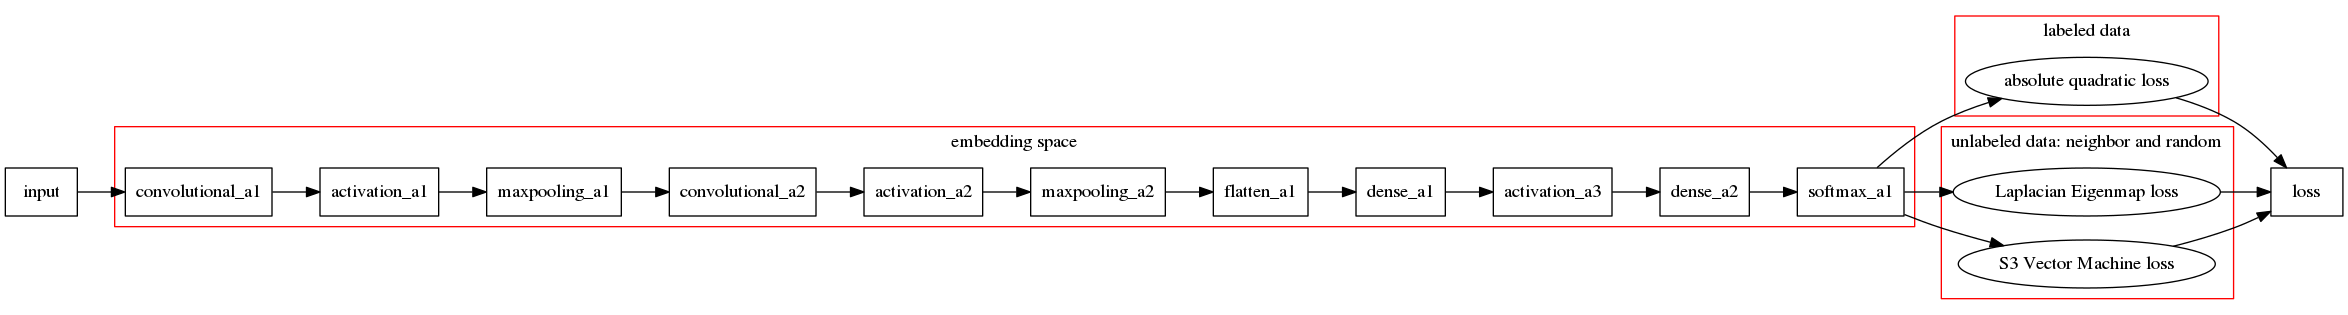
\includegraphics[width=\linewidth]{fig10.png}
\end{center}

The feature mapping(neural network) is the same for labeled and unlabeled data. But because of the absence of label, loss function would be different.

$$ \sum_{i=1}^M l (f(x_i), y_i) + \lambda \sum_{i,j=1}^{M+U} L(f(x_i), f(x_j), W_{i,j}) $$
\end{frame}
%------------------------------------------------------------
\begin{frame}
\frametitle{For labeled data}

The fisrt term is labeled data loss:

$$ \sum_{i=1}^M l (f(x_i), y_i) $$

At first I used hinge loss:

$$ \mathcal{L}(y, y_t) = \max(0, 1 - y_t \cdot y) $$

But later I found absolute quadratic loss maybe better:

$$ \mathcal{L}(y, y_t) = \max(0, 1 - |y_t \cdot y|)^2 $$

table, page 5
\end{frame}
%------------------------------------------------------------
\begin{frame}
\frametitle{For unlabeled data}

The paper proposed 3 embedding algorithms:

\begin{enumerate}
\item Multidimensional scaling \\ 

$$ L(f(x_i), f(x_j), W_{i,j}) = (||f_i - f_j|| - W_{ij})^2 $$
\item ISOMAP  \\
\item Laplacian Eigenmaps  \\ 

$$ \sum_{i,j} L(f(x_i), f(x_j), W_{i,j}) = \sum_{i,j} W_{ij} ||f_i - f_j||^2 $$
\item Siamese Networks \\

$$ L(f_i, f_j , W_{ij}) = \max(0, m - ||f_{i} - f_{j}||_2)^2,  \text{ if } W_{ij} = 0 $$
\end{enumerate}

$W_{ij}$ indicates the neighbor relationship.

\end{frame}
%------------------------------------------------------------
\begin{frame}
\frametitle{Most Computation}

$W_{ij}$\\

\bigskip

Different $W_{ij}$ would take very different time.\\

\begin{enumerate}
\item k-N \\ 
slow\\
\item pixel  \\
fast\\
\end{enumerate}

This is because k-N involves computing distance and ordering:\\

$$ \sqrt{ (\mathbf{x_1} - \mathbf{x_2})^T (\mathbf{x_1} - \mathbf{x_2}) } $$

\end{frame}
%------------------------------------------------------------
\begin{frame}
\frametitle{Difficulty of Implementation}

\begin{enumerate}
\item Loss \\ 
It is difficult to represent $W_{ij}$ in tensorflow. Code trick ...
\item Batch  \\
This algorithm cannot perform batch computation in tensorflow, though its loss is written as:\\

$$ \sum_{i=1}^M l (f(x_i), y_i) + \lambda \sum_{i,j=1}^{M+U} L(f(x_i), f(x_j), W_{i,j}) $$

\item Weight Reusing\\
Define layers outside function in Keras.\\
\end{enumerate}

\end{frame}
%------------------------------------------------------------
\begin{frame}
\frametitle{Improve: Add S3VM loss}

The loss described in paper:

$$L_{\text{supervised}} + \alpha L_{\text{manifold}} $$ 

But we can add loss based on cluster to compare:

$$L_{\text{supervised}} + \alpha L_{\text{manifold}} + \beta L_{\text{cluster}}$$ 

s.t. $\beta +\alpha=1$.

I  used S3VM loss here:

$$ \sum_{\text{labeled}} \max(0, 1 - y_i f(x_i)) + \lambda_1 + ||h||^2_{\mathcal{HK}} + \lambda_2 \sum_{\text{unlabeled}}\max(0, 1 - |f(x_i)|)$$

Preference: table, page 4

\end{frame}
%------------------------------------------------------------
\begin{frame}
\frametitle{Careful points}

One-hot label ...... nan problem\\

Distance:\\

good LE:\\

$$ \sum_{ij} L(f_i, f_j, W_{ij}) = \sum_{ij} W_{ij} ||f_i - f_j||^2 $$


bad LE:\\

$$ \sum_{ij} L(f_i, f_j, W_{ij}) = \sum_{ij} W_{ij} ||f_i - f_j|| $$

good SN:\\

$$ L(f_i, f_j , W_{ij}) = \max(0, m- ||f_i - f_j||_2)^2,  \text{ if } W_{ij} = 0 $$

bad SN:\\

$||f_i - f_j||_2 = (f_i - f_j)^T(f_i - f_j)$


\end{frame}
%------------------------------------------------------------
\begin{frame}
\frametitle{Improve}

\begin{enumerate}
\item Change Embedding Algorithm \\ 

Use Laplacian Eigenmaps instead of Siamese Networks. Table, page 5

\item Absolute Quadratic Loass  \\

$$ \mathcal{L}(y, y_t) = \max(0, 1 - |y_t \cdot y|)^2 $$

table, page 5\\

\item Neighbor Radius\\
R = 1,2,3: table, page 5\\

\item Auxiliary EmbedCNN\\
\end{enumerate}

\end{frame}
%------------------------------------------------------------
\begin{frame}
\frametitle{Improve}

NN Auxiliary:

\begin{center}
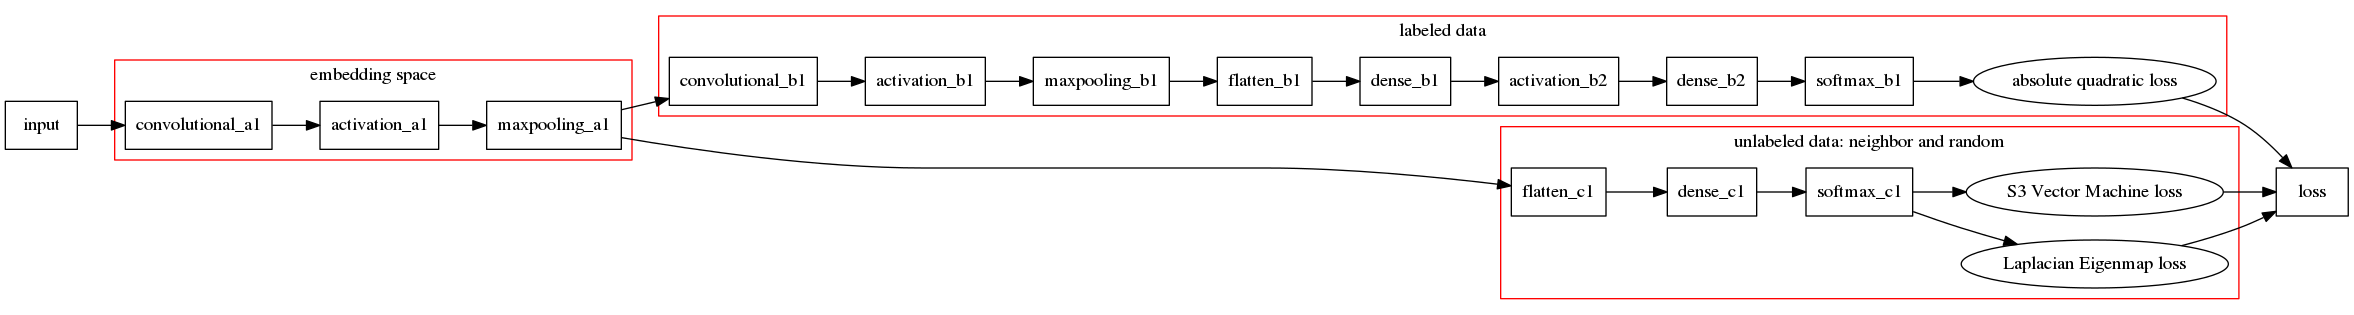
\includegraphics[width=\linewidth]{fig11.png}
\end{center}

CNN Auxiliary:

\begin{center}
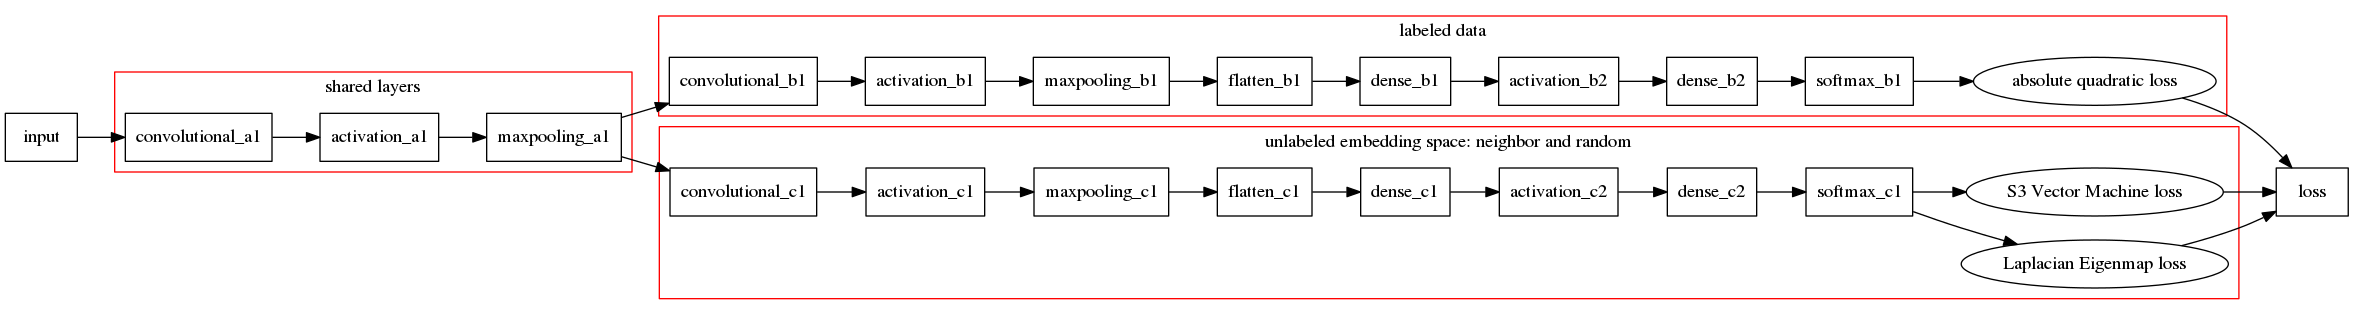
\includegraphics[width=\linewidth]{fig12.png}
\end{center}

\end{frame}
%------------------------------------------------------------
\begin{frame}
\frametitle{S3VM}

Memory Problem\\

Cannot find Multi-label Semi-supervised SVM\\

\end{frame}
%------------------------------------------------------------
\begin{frame}
\frametitle{DRBM}

Structure and loss:\\

$$ \mathcal{L}_{\text{semi-sup}} (\mathcal{D}_{\text{train}} , \mathcal{D}_{\text{unlab}}) = \mathcal{L}_{\text{TYPE}}(\mathcal{D}_{\text{train}}) + \beta \mathcal{L}_{\text{unsup}} (\mathcal{D}_{\text{unlab}}) $$


$$ = -\sum_{i=1}^{|\mathcal{D}_{\text{train}}|} \log p(y_i | \mathbf{x_i}) - \beta \sum_{i=1}^{|\mathcal{D}_{\text{unlab}}|} \log p(\mathbf{x_i}) $$

or 

$$ = -\sum_{i=1}^{|\mathcal{D}_{\text{train}}|} \log p(y_i | \mathbf{x_i}) -\alpha \sum_{i=1}^{|\mathcal{D}_{\text{train}}|} \log p(y_i , \mathbf{x_i}) - \beta \sum_{i=1}^{|\mathcal{D}_{\text{unlab}}|} \log p(\mathbf{x_i}) $$

\end{frame}
%------------------------------------------------------------
\begin{frame}
\frametitle{DRBM - Implementation}

Turn the gradient for U, d zero:\\

code, line 322

\end{frame}
%------------------------------------------------------------
\begin{frame}
\frametitle{Other Algorithms}

\begin{enumerate}
\item Label Spreading \\ 

\item Ladder Network \\

\end{enumerate}

\end{frame}
\end{document}